\newpage
%%%%%%%%%%
% TESTING PAUSE MEASUREMENT
%%%%%%%%%%
\subsection{Test 2: Testing Pause Length Measurement}
These tests were done to determine how accurate the pause length measurements were. 
%Millisecond was chosen as the time frame because it provided a sufficient level of detail for the experiments. 
%Although finer grain detail would be good, this was all that was required for this thesis.

\paragraph{\underline{Test 2.1: Four Constructed Pauses - [1s, 10ms, 1ms, 3s]}}
\begin{description}
	\item[\underline{Test:}] This test aimed to see how well calpy detects different granularities of pauses. 
						The same audio from test 1.1 was used, the pauses were 1s, 10ms, 1ms and 3s respectively.
						The same utterance is used throughout the recording.
	\item[\underline{File:}] data/pause\_test/timing/nine\_constructed\_pauses.wav
	\item[\underline{Result:}] The output was 10, 1, 30. Indicating calpy is digitising pauses only down to the 100ms level, 
						but still recognising a pause is present (e.g. the 10ms pause still being recognised).
\end{description}
\begin{figure}[h]
	\center
	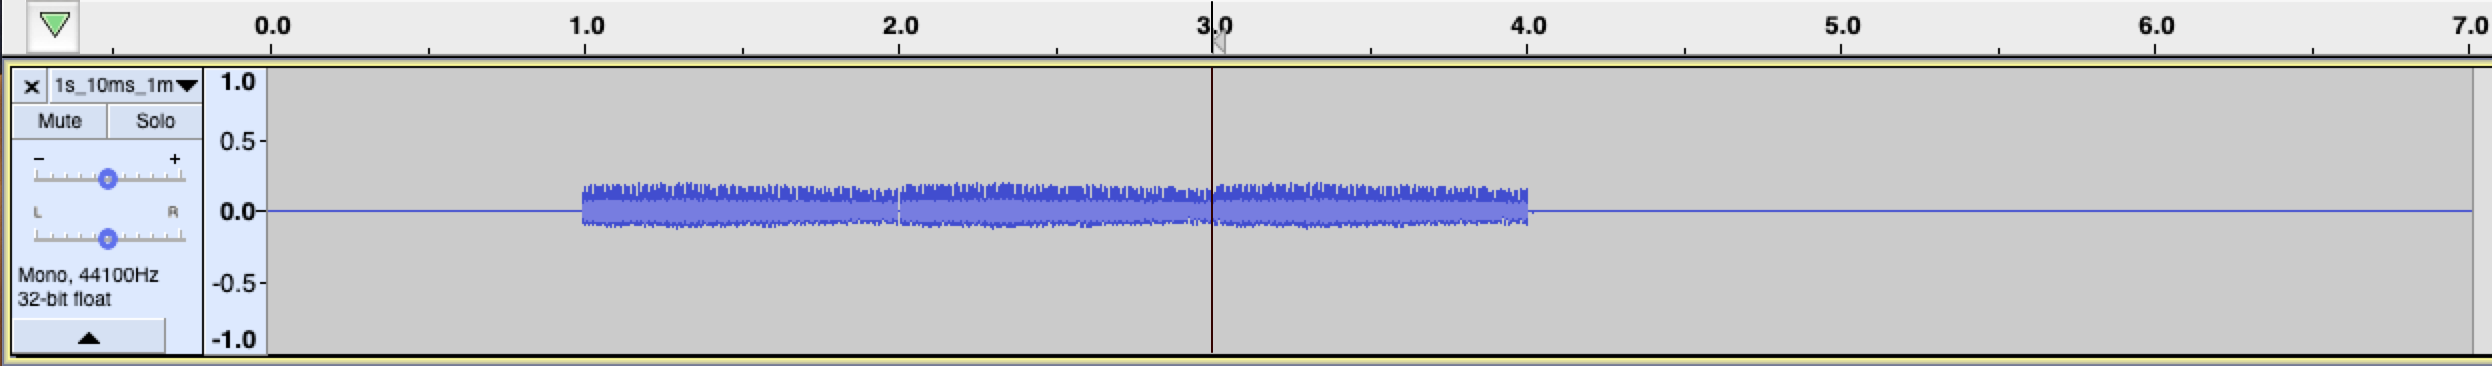
\includegraphics[scale=0.3]{src/main-matter/results/preliminary-testing/detection/1s_10ms_1ms_3s}
	\caption{Four Constructed Pauses of [1s, 10ms, 1ms, 3s]}
	\label{fig:021}
\end{figure}



\paragraph{\underline{Test 2.2: Four Constructed Pauses - [1s, 20ms, 1ms, 3s]}}
\begin{description}
	\item[\underline{Test:}] This test aimed to confirm the digitisation from test 2.1 was correct 
						The same audio from test 2.1 was used, except the 10ms pause was extended to 20ms.
	\item[\underline{File:}] data/pause\_test/timing/nine\_constructed\_pauses.wav
	\item[\underline{Result:}] The output was 10, 1, 30.
\end{description}
\begin{figure}[h]
	\center
	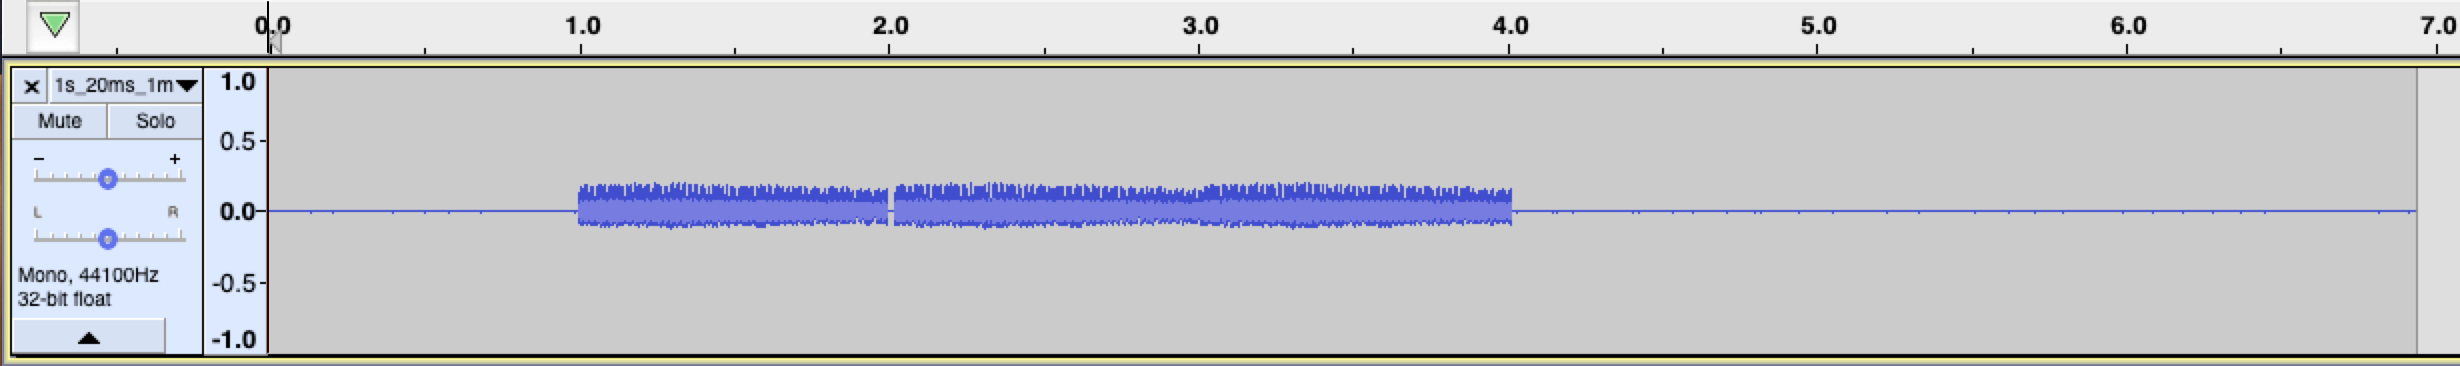
\includegraphics[scale=0.3]{src/main-matter/results/preliminary-testing/detection/1s_20ms_1ms_3s}
	\caption{Four Constructed Pauses - [1s, 20ms, 1ms, 3s]}
	\label{fig:022}
\end{figure}


\paragraph{\underline{Test 2.3: Four Constructed Pauses - [500ms, 40ms, 1ms, 3s]}}
\begin{description}
	\item[\underline{Test:}] This test aimed to further test the digitisation values returned.
						The same audio from test 2.2 was used, except the 20ms pause was extended to 40ms
						and the 1s pause was reduced to 500ms.
	\item[\underline{File:}] data/pause\_test/timing/nine\_constructed\_pauses.wav
	\item[\underline{Result:}] The output was 5, 1, 30.
\end{description}
\begin{figure}[h]
	\center
	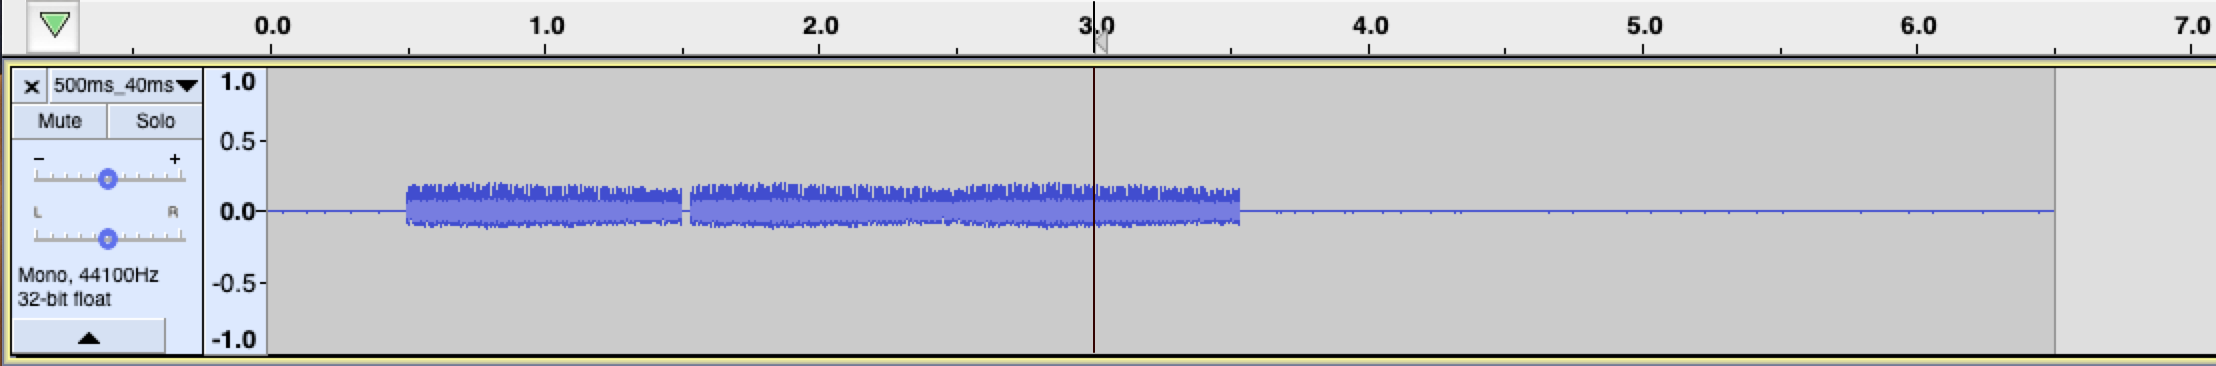
\includegraphics[scale=0.3]{src/main-matter/results/preliminary-testing/detection/500ms_40ms_1ms_3s}
	\caption{Four Constructed Pauses - [500ms, 40ms, 1ms, 3s]}
	\label{fig:023}
\end{figure}


\paragraph{\underline{Test 2.4: Four Constructed Pauses - [500ms, 80ms, 1ms, 3s]}}
\begin{description}
	\item[\underline{Test:}] This test aimed to further test the digitisation values
						The same audio from test 2.3 was used, except the 40ms pause was extended to 80ms.
	\item[\underline{File:}] data/pause\_test/timing/nine\_constructed\_pauses.wav
	\item[\underline{Result:}] The output was 5, 1, 30.
\end{description}
\begin{figure}[h]
	\center
	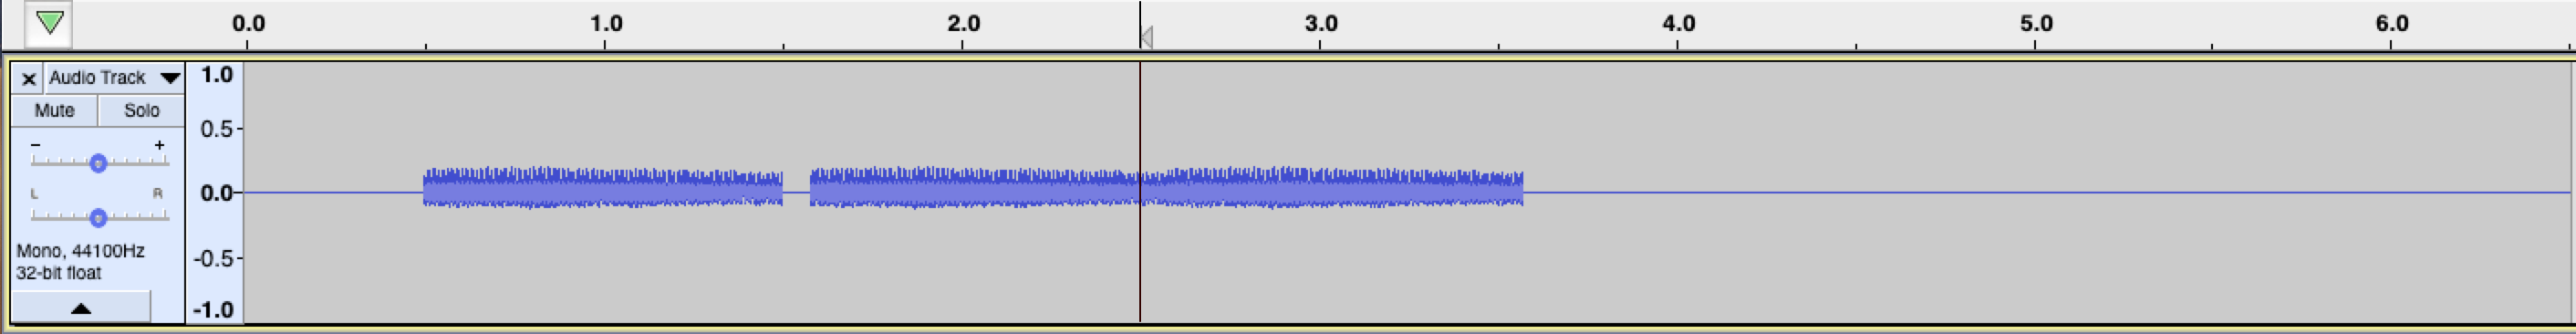
\includegraphics[scale=0.3]{src/main-matter/results/preliminary-testing/detection/500ms_80ms_1ms_3s}
	\caption{Four Constructed Pauses - [500ms, 80ms, 1ms, 3s]}
	\label{fig:023}
\end{figure}

\paragraph{\underline{Test 2.5: Four Constructed Pauses - [500ms, 40ms, 9ms, 3s]}}
\begin{description}
	\item[\underline{Test:}] This test aimed to further test the digitisation values
						The same audio from test 2.3 was used, except the 1ms pause was extended to 9ms.
	\item[\underline{File:}] data/pause\_test/timing/nine\_constructed\_pauses.wav
	\item[\underline{Result:}] The output was 5, 1, 1, 30.
\end{description}
\begin{figure}[h]
	\center
	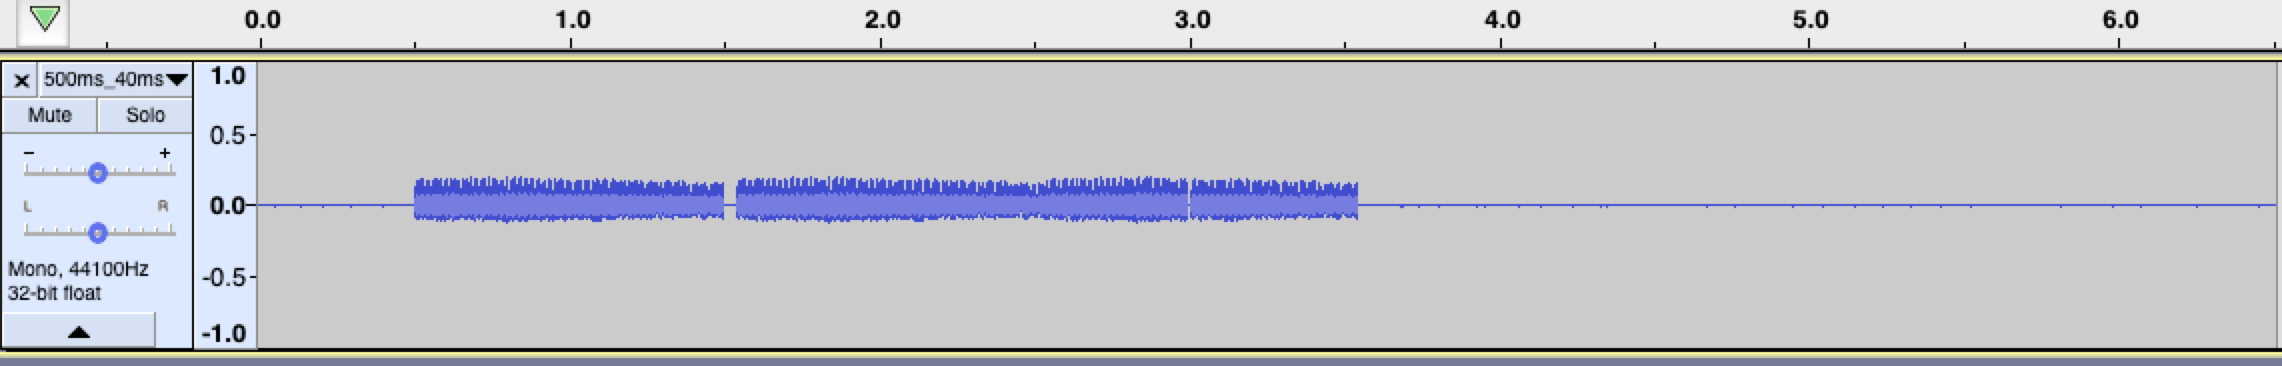
\includegraphics[scale=0.3]{src/main-matter/results/preliminary-testing/detection/500ms_40ms_9ms_3s}
	\caption{Four Constructed Pauses - [500ms, 80ms, 1ms, 3s]}
	\label{fig:023}
\end{figure}

\subsubsection{Test 2 Results}
The results showed that digitisation is done at the 100ms level but that pauses can be detected down at the 9ms level